\documentclass[12pt]{article} % article class, 12pt font

% load any packages you need for more custom stuff
\usepackage[margin=1in]{geometry} % set 1-inch margins
\usepackage{setspace}\doublespacing % set double spacing
\usepackage[superscript]{cite} % superscript numeric in-line citations
\usepackage{indentfirst} % indent the first paragraph of each section
\usepackage{graphicx} % enable displaying png format graphs
\usepackage{csvsimple} % enable importing tabular data
\usepackage{booktabs} % enable formulating tables
\usepackage{tabto} % allows you to tab stuff
% \newcommand\tab[1][1cm]{\hspace*{#1}}

% set title stuff
\title{Row Row Row Your Boat}
\newcommand{\authors}{Eli Sylvia-Lourde}
\author{Math 114 Mathematical Modeling\\St. Mary's College}
\date{March 8, 2019}

\begin{document}

% create title stuff
\hfill\authors % write the authors right-aligned
%\vspace{-0.5in} % reduce space before title
{\let\newpage\relax\maketitle} % print title

\section*{Problem Statement}
—If you have been to a rowing regatta, you may have observed that the more oarsmen there are in a boat, the faster the boat travels. Investigate whether there is a mathematical relationship between the speed of a boat and the number of crew members. Consider the following assumptions (partial list) in formulating a model:

\begin{enumerate}
\item
The total force exerted by the crew is constant for a particular crew throughout the race.
\item
The drag force experienced by the boat as it moves through the water is proportional to the square of the velocity times the wet surface area of the hull.
\item
Work is defined as force times distance. Power is defined as work per unit time.
\end{enumerate}
Hint: When additional oarsmen are added to a shell, it is not obvious whether the amount of force is proportional to the number in the crew or the amount of power is proportional to the number in the crew. Which assumption appears the most reasonable? Which yields a more accurate model?

\section*{Data}
{\centering
\csvautobooktabular{boat_data.csv}
\\}

Distance is in meters and time is in minutes:seconds

\section*{Commentary}

For this problem we are deciding to make a model that will return the race time of a team given how many people are in the boat and what race the team is currently running. Looking at the data, we can see that time increases as the number of races performed increases. This suggests that those that are participating in the race are getting more tired as they participate in more races. Depending on the size of the team, different energy systems of the teammembers are being exhausted to a different degree. Due to the lack of data, we will assume that teams of size 1-2 tire in a way that is different than teams of size 4-8. With respect to the measure of force vs power, the measure of force will not be useful when trying to model the fatigue of teams, as the amount of force required to complete the race has not changed, even though the time will. If we use power, we will be better able to see how the team fatigued as they participated in consecutive races.

Given this discussion, we will be transforming the data above from time to power. We will create two models, one that predicts the first race time, and another that predicts the rate at which the teams will fatigue. Our model will support team sizes of 1,2,4,8 and races numbers of 1-6.

\section*{Power Data}

We are told from our list of assumptions that power is work per unit time, work is force times distance, and the force acted on the boat in order to move it is $force = k*v^{2}*SA_{hull}$, $v = distance/time$. We can reduce the equation in the following way:

\[power = work/time\]
\[power = (force*distance)/time\]
\[power = ((k*v^{2}*SA_{hull})*distance)/time\]
\[power = ((k*(distance/time)^{2}*SA_{hull})*distance)/time\]
\[power = ((k*(distance^{2}/time^{2})*SA_{hull})*distance)/time\]
\[power = ((k*(distance^{3})*SA_{hull}))/time^{3}\]
\[power = \frac{k*distance^{3}*SA_{hull}}{time^{3}}\]

For the sake of simplicity, we will allow k to be one. Also for the sake of simplicity, we will allow $SA_{hull}$ to be equal to the number of people in the boat. To actually find k, we would most likely need more data. To get a more accurate value of $SA_{hull}$, we'd have to get the size of the boat used for a crew of size 1,2,4,8, as the boat sizes are not constant, as well as the data needed to calculate how far below the water the boat would be, which would require some more physics as well as data to properly predict. Setting $k=1$ and $SA_{hull} =$ the number of people in the boat, we get the following data:
\\
\section*{Power Data}
{\centering
\csvautobooktabular{power_boat_data.csv}
\\}

\section*{Model 1: The first race}
The first model that we are creating will output how much power a crew will exert during a race given the number of people in the boat. Since most of the data we have is based upon subsequent races, we will only be using data from race 1. When thinking about what kind of model we should fit to our data, we should consider the power that each rower brings to the team. For the sake of simplicity, we may assume that all rowers output the same power, and that the only people in the boat are actively rowing. This means that none of the people in the boat are acting as the coxswain, a position in boats of larger teams whose responsibility it is to steer the boat and set the tempo instead of doing any actual rowing. Following these assumptions, we assume that the power output of every athlete is the same and that every athlete tires at a uniform rate. Given these assumptions, we can conclude that every additional athlete increases the boat's ability to output power by a constant number (e.g power output of boat with n rowers = $P_{n}$, $P_{n+1}=P_{n}+C$). While other regression techniques exist that yield a smaller least squares value, a linear regression most aptly matches our assumptions.

Using polyfit from the library numpy, we get $104.383x-188.038$, which has a least squares of 604406.716.

% 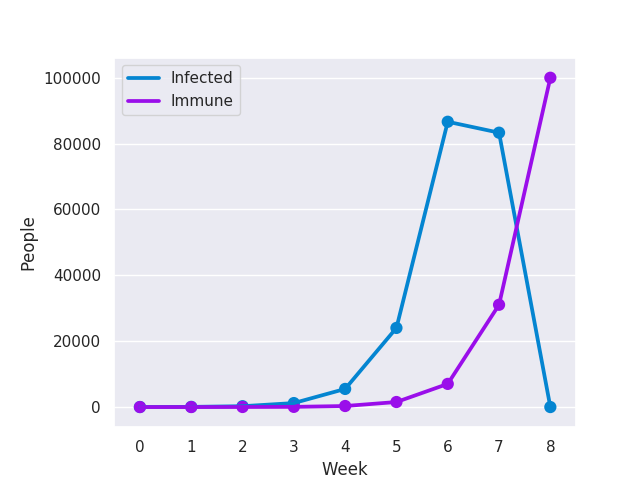
\includegraphics{humans_win.png}
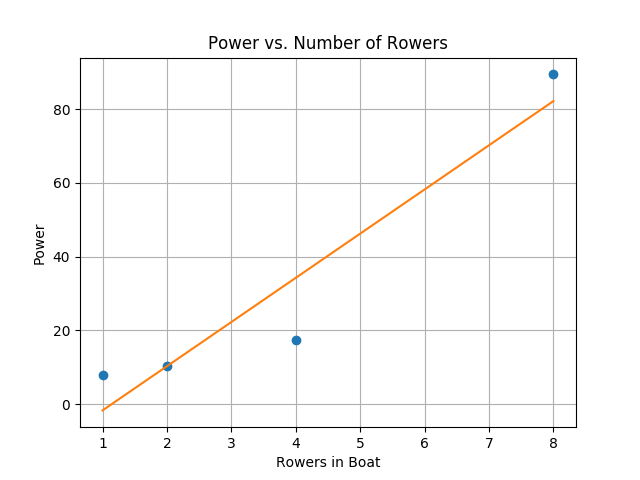
\includegraphics{Linear_Line_Done_Correctly.png}

\section*{Model 2: Fatigue}
Our goal for this model is to calculate how an individual tires as they consecutively race, and then use the race number, as well as the number of people in the boat to determine how much slower the team will perform as they continue to race. In order to calculate how a person slows as they race we will look at the difference in power outputs at a certain race. We will then divide this difference by the number of people in the boat, and then average these values to determine how much of a decrease we might expect for a given race number.

\[Diff(x) = (Race_{x-1}-Race_{x})/(Size of Crew)\]

Where the first difference is equal to the first race time minus the second race time divided by the number of people in the boat. Diff 1, People in Boat 8, for example, is equal to $(678.536-715.607)/8 = -4.634.$

\section*{Fatigue Data}

{\centering
\csvautobooktabular{diff.csv}
\\}
_
\\

Looking at the data, a boat with 8 people has a very different diff than any other boat. This leads me to hypothesize about the fluidity of the rower's strokes in the boat of 8 people. If the uniformity of the rower's stroke affects the race time, and a rower might struggle to operate in uniformity if they are tired, and it is harder for multiple rowers to row in uniformity, especially if they are tired, then the 8-person boat might have such a high diff when compared to boats that have less people in them. Due to lack of data, this can neither be proven nor disproven, so we will use the data despite the fact that it is visibly different than the other boats.

\section*{Fatigue to Expect }

{\centering
\csvautobooktabular{fatigue_data.csv}
\\}

\\
_




Since the force that is applied is constant, we can check how good our approximation is using least squares on the force data. We now take the number of people in the boat, and what race they are running, and use this to predict the power output for their race. This is done with the linear regression that was performed earlier in the project. Depending on race that the rowers are on, we then subtract the neccessary fatigue constant from that result. If they are on race 2, we subtract $2.028$, if they are on race 3, we subtract $2.469$, etc. To summarize, we have the following equation:

    \[a = 104.38298143764881\]
    \[b = -188.03775163057534\]
    \[p(x,r)=ax+b -F_{r} \]
  Where $p(x,r)$ is the expected power of a boat of $x$ rowers after $r$ races.
\\This modeling strategy returns a least squares of $267639.0378$ and the following tables and visualization.





\section*{Actual Peformance}

{\centering
\csvautobooktabular{expected.csv}
\\}

\section*{Predicted Performance}

{\centering
\csvautobooktabular{y_hat.csv}
\\}


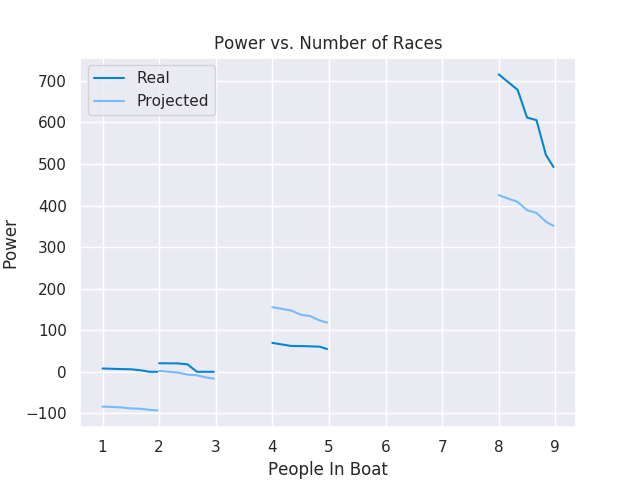
\includegraphics{modeling_results.png}

This visualization is purposefully confusing. The number of people in the boat doesn't increase, the teams just participate in new races. This was done to properly visualize how the power output of the teams is affected by the participation in consecutive races.

\section*{Conclusion}
Though the effectivness of the modeling was hamstrung by the lack of data, this project does a very good job of showing the different assumptions and thought processes that are used when walking through a data science problem. If I did this project again, I would use an exponential curve to model the expected power output and I would make a different set of fatigue constants for every race. This would result in a much better model, however there is a good chance that this model would suffer from overfitting. If there was more data, I would love to test my assumptions about fatigue and power output given the number of people in the boat. Looking forward to more complicated, data-heavy projects. I used main.py and fatigue.py to generate the different data/visualization/models discussed in this report. They are  


\end{document} % this ends your document
